\begin{savequote}[75mm] 
Nulla facilisi. In vel sem. Morbi id urna in diam dignissim feugiat. Proin molestie tortor eu velit. Aliquam erat volutpat. Nullam ultrices, diam tempus vulputate egestas, eros pede varius leo.
\qauthor{Quoteauthor Lastname} 
\end{savequote}

\chapter{Implementation}
\label{chapterfive}


The platform at hand uses a service-oriented architecture. The base of the platform supports a limited number of actions. The capabilities of the platform can be further expanded through developed services. Communications between the platform and all clients is done through MQTT. This is a lightweight machine to machine messaging protocol for use on top of the TCP/IP protocol. The services which extend the cloudlet can be physically located on the mobile device or the device that hosts the cloudlet. Figure \ref{fig:protocol} shows the physical location of services in the cloudlet. The services which extend the cloudlet need to use raw sockets. That is, they should create a server using raw sockets and not use the MQTT protocol as it has limitations in the message payload size. When a user request a service, they should be provided an ip and port. Those details will be used to communicate.


\begin{figure}
\centering
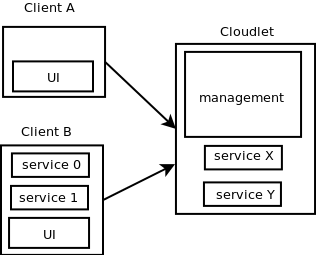
\includegraphics[scale=0.5]{figures/protocol}
\caption{Physical location of services}
\label{fig:protocol}
\end{figure}

\subsection{Component structure}

Figure \ref{fig:objstruc} shows the class hierarchy and components which make the cloudlet. The responsibility of the controller class, as it's name suggests, is to control the cloudlet. It is the entry point for the system.
Its responsibility is to receive a port number and start the mosquitto event handler (thus mosquitto) and the communication handler on the specified port. The communication handler sets up the appropriate channels which are
used for sending requests to the cloudlet. These channels allow joining a cloudlet, requesting a service list  and requesting a connected user list from the clients. The communication handler uses the service manager and
user manager for most of the actions. The mosquitto event handler class is designed to extend mosquitto. It detects client connections and disconnections. The service manager is responsible for keeping track of available
services, loading them and other management taks for services. The user manager keeps track of online users and the services they are using.

\begin{figure}
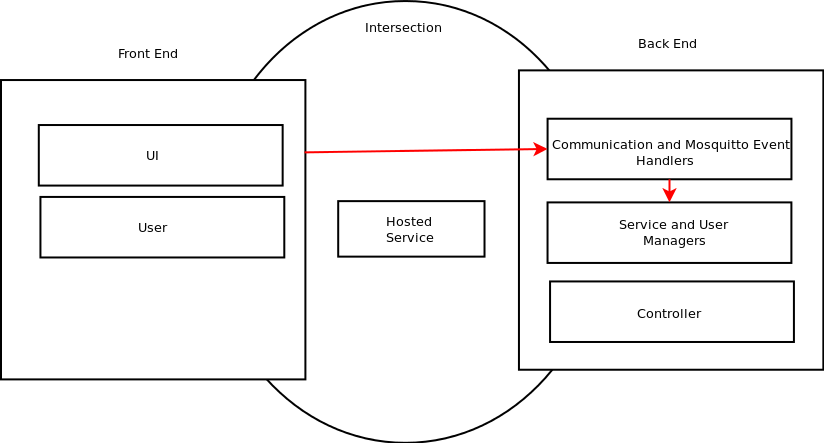
\includegraphics[scale=0.4]{figures/newcomponentstructure}
\caption{Classes that make up cloudlet. Red lines show communication between components.}
\label{fig:objstruc}
\end{figure}

\subsubsection{Mosquitto Event Handler}
Mosquitto, as stated above in section \ref{communication}, is an open-source broker that implements version 3.1 of the MQTT protocol. Mosquito does not have a mechanism that allows applications to hook into such that they alerted of connections and disconnections. However, the application writes messages on the standard error stream when there is a connection or disconnection. The mosquitto event handler class is responsible for starting a mosquitto process and
capturing it's error stream. The data on that stream is used to alert the communication handler of connections and disconnections. The readiness of the standard error stream, that is the availability of data on that
stream, is determined by using the ``select" system call which is available for all Unix-like and POSIX-compliant operating systems.


\subsubsection{Service}
The service can be located on the raspberry pi or on the phone. This is illustrated in figure \ref{fig:objstruc}. The service class contains information about a service such as it's name and description. It also handles service requests which have already been
granted by the user manager and service manager. The implementation of the services on the cloudlet requires communication between service and client to not go through the communication handler. The clients are
allocated an IP and port to connect to using TCP, when they request a service. This is because services cannot use the mosquitto channels for communication as channels require the payload to not exceed 260MB.
The mobile device has the ability to host services therefore it can advertise hosted services. One can request a list of services, however, it is possible that the name is not descriptive enough. Therefore each
service has a string which acts as it's metadata. The string is as follows:

\begin{lstlisting}
``Name=somename;CloudletV=somenumber;
Description=somedescription.;authors=somename;
Copyright=Copyright someyear somename;
Website=https://example.com".
\end{lstlisting}

\noindent This format allows the client to be able to view details of the services. In addition, since this is sent as one string. It removes the need for the client to request various fields which it needs.